\documentclass[12pt,a4paper]{article}
 
% ── Geometry & font ──────────────────────────────────────────────────────────
\usepackage[top=1.5cm,bottom=1.5cm,left=1.5cm,right=1.5cm]{geometry}
\usepackage[T1]{fontenc}
\usepackage[utf8]{inputenc}
\usepackage{lmodern}
\setlength{\parskip}{4pt}
\setlength{\parindent}{0pt}
\renewcommand{\baselinestretch}{1.0}
 
% ── Math & tables ─────────────────────────────────────────────────────────────
\usepackage{amsmath,amssymb}
\usepackage{amsthm}
\usepackage{booktabs}
\usepackage{array}
 
% ── Graphics & colors ─────────────────────────────────────────────────────────
\usepackage{graphicx}
\usepackage{xcolor}
\usepackage{tikz}
\usepackage{pgfplots}
\pgfplotsset{compat=1.18}
 
% ── Sections: tighter spacing ─────────────────────────────────────────────────
\usepackage{titlesec}
\titlespacing{\section}{0pt}{8pt}{4pt}
\titlespacing{\subsection}{0pt}{6pt}{2pt}
\titleformat{\section}{\large\bfseries}{}{0em}{}[\titlerule]
\titleformat{\subsection}{\normalsize\bfseries}{}{0em}{}
 
% ── Hyperlinks ────────────────────────────────────────────────────────────────
\usepackage[hidelinks]{hyperref}
 
% ── Header ────────────────────────────────────────────────────────────────────
\title{Derivatives - Group P}
\author{\parbox{0.9\textwidth}{\centering Petrit Arifi (362548), Adam Ait Bousselham (356365), Florian Dinant (361013), Mohamed Mamouri (362231)}}
\date{May 2026}

\begin{document}
\maketitle

\section*{Part 1 --- History of the Dividend Derivatives Market}
 
Dividends have long been an implicit component of equity prices, but they were not
traded as standalone risk factors until the early 2000s.
Before that, dividend exposure could only be gained indirectly: by holding equities and
receiving cash distributions, or by entering total-return vs.\ price-return swap
structures with investment banks.
 
The first liquid OTC dividend swap market developed around 2002--2004, driven by
structured products desks that needed to delta-hedge dividend risk embedded in
long-dated equity derivatives (such as constant-proportion portfolio insurance products
and life-insurance wrappers with guaranteed floors).
Banks realized they were systematically short dividends via these hedges, and began
seeking natural counterparts: pension funds and other income-oriented investors who were
willing to receive fixed dividends in exchange for paying floating realised dividends.
 
The move to listed markets came in 2008, when Eurex launched the first
\textbf{Euro Stoxx 50 Annual Dividend Index Futures} (ticker: \texttt{FEXD})~\cite{eurex}.
The timing, just as the 2008--2009 financial crisis was unfolding, proved consequential:
the market observed a dramatic repricing of near-term dividend expectations as corporates
cut payouts aggressively, immediately demonstrating that dividends carry substantial
independent risk.
By 2012--2014, Eurex had extended the product suite to single-stock dividend futures
on major European names (Total, Allianz, BASF, \ldots) and a growing number of maturities.
Options on dividend futures (dividend options) followed, enabling the construction of a
full implied dividend surface.
Open interest grew steadily, reaching several hundred thousand contracts by the early
2020s, with the Euro Stoxx 50 contract as the most liquid single market.
 
% ═══════════════════════════════════════════════════════════════════════════════
\subsection*{Main Eurex Dividend-Related Derivatives}
 
\subsubsection*{Dividend Index Futures}
 
The flagship product is the \textbf{Euro Stoxx 50 Dividend Index Future} (Eurex:
\texttt{FEXD}).
Each contract is written on the \emph{Euro Stoxx 50 Dividend Index}, which accumulates
the gross ordinary cash dividends paid by all 50 index members during a given
calendar year (the \emph{reference year}).
At expiration (third Friday of December of the reference year), the contract settles
in cash against the realised index-year dividend.
The contract multiplier is 100 EUR per index point.
 
\smallskip
\textbf{How it works.} The price of the December-$T$ contract reflects the market
consensus for the sum of all ordinary dividends paid in year $T$:
\[
F_t^{\text{div}}(T) \;=\; E_t^{\mathbb{Q}}\!\left[\,\sum_{i\in\text{SX5E}}\,D_i^T\,\right],
\]
where $D_i^T$ is the dividend paid by member $i$ in year $T$ (adjusted for index weights
and divisor). Before expiry, the contract can be bought, sold, or rolled exactly like a
standard equity index future.
 
\smallskip
\textbf{Single-stock variants.} Eurex also lists dividend futures on individual
constituents (e.g.\ \texttt{BASFD} for BASF). These are cash-settled against the
ordinary \emph{gross} dividend per share paid over the reference period, letting
investors trade company-specific dividend expectations. The contract size (shares per
contract) is set per underlying.
 
\subsubsection*{Dividend Index Options}
 
Eurex offers European-style options written directly on the Euro Stoxx 50 Dividend Index
Future. They carry the same December maturities and allow the construction of:
a dividend implied volatility surface, optionality on dividend surprise events
(AGM seasons, special dividends), and volatility-of-dividend trading strategies.
 
\smallskip
\textbf{Key use cases across contract types.}
 
\begin{center}
\small
\begin{tabular}{p{3.8cm}p{4.2cm}p{4.8cm}}
\toprule
\textbf{Contract} & \textbf{Typical buyer} & \textbf{Objective} \\
\midrule
Div.\ index future (long)
  & Structured products desk
  & Hedge short-dividend exposure embedded in capital-protected notes \\[3pt]
Div.\ index future (short)
  & Asset manager / pension fund
  & Lock in high future dividends; monetise dividend risk premium \\[3pt]
Div.\ index option (call)
  & Macro hedge fund
  & Bet on dividend recovery after a downturn \\[3pt]
Div.\ index option (put)
  & Corporate treasury / insurer
  & Protect income projections against dividend cuts \\[3pt]
Single-stock div.\ future
  & Event-driven fund
  & Play a specific company's payout decision \\
\bottomrule
\end{tabular}
\end{center}
 
% ═══════════════════════════════════════════════════════════════════════════════
\subsection*{Why Dividend Futures Exist}
 
\subsubsection*{Dividends as an independent risk factor}
 
In classical equity valuation, the price of a stock equals the present value of all
future dividends~\cite{hull}.
Yet until listed dividend futures existed, investors had no way to \emph{separately}
express a view on dividends without simultaneously taking on price risk (capital gains
risk).
Dividend futures complete the market by isolating the dividend component:
 
\smallskip
\textit{Long equity = long dividends + long capital gains risk.}
 
\smallskip
A long dividend future, taken on its own, already provides exposure to future dividends
without the price (capital-gains) risk of the index.
Conversely, a portfolio manager who holds equities purely for income can \emph{lock in}
projected dividend cash flows by selling dividend futures, transforming uncertain income
into a contractually fixed stream, analogous to converting a floating-rate bond into
a fixed one via an interest-rate swap.
 
\subsubsection*{Structural demand: the hedging motive of banks}
 
The existence of the market was initially driven by the hedging needs of bank trading
desks.
Long-dated equity derivatives (barrier notes, CPPI products, guarantee-embedded
insurance contracts) implicitly embed short-dividend exposure: when dividends are paid,
the stock price drops by roughly the dividend amount on the ex-date, reducing the
value of call-heavy payoff profiles.
Desks that are long these products are therefore \emph{short} dividends and need to
buy them back in the market.
Dividend futures provide a transparent and liquid venue for this hedging.
 
\subsubsection*{The dividend risk premium}
 
Dividend risk can also carry a \textbf{risk premium}. Since dividends tend to fall in
bad economic states, investors who take long dividend exposure require compensation for
bearing this risk; as a result, dividend futures have tended to trade \emph{below}
investors' statistical expectations of future realised dividends~\cite{vbk}.
This premium has attracted carry-oriented investors (hedge funds, asset managers) who
buy dividend futures as a systematic alternative risk premium strategy, deepening
liquidity.
 
% ═══════════════════════════════════════════════════════════════════════════════
\subsection*{The Equity Term Structure and Its Relation to Dividend Futures}
 
\subsubsection*{Definition}
 
The \textbf{equity term structure} describes how the value of an index's dividends is
distributed across future horizons: for each maturity $T$ it gives the present value
today of the dividends expected to be paid up to that date~\cite{vbk}.
Dividend futures are the traded instruments that reveal it: each annual contract prices
the dividends of one calendar year, so the strip of dividend futures across maturities
directly maps out this curve, exactly as the yield curve is represented by bond prices
across maturities.
 
Formally, the time-$t$ value of dividends paid in $[t,T]$ is:
\[
\mathcal{D}_t(T) \;=\; S_t - k\,B_t(T) - C_t(T,k) + P_t(T,k), \quad \forall k,
\]
where $B_t(T)$ is the zero-coupon price, and $C_t, P_t$ are European call/put prices
at strike $k$.
Each annual dividend futures contract essentially prices one \emph{slice} of this term
structure (the dividends attributable to one specific calendar year).
 
\subsubsection*{Shape and interpretation}
 
\begin{center}
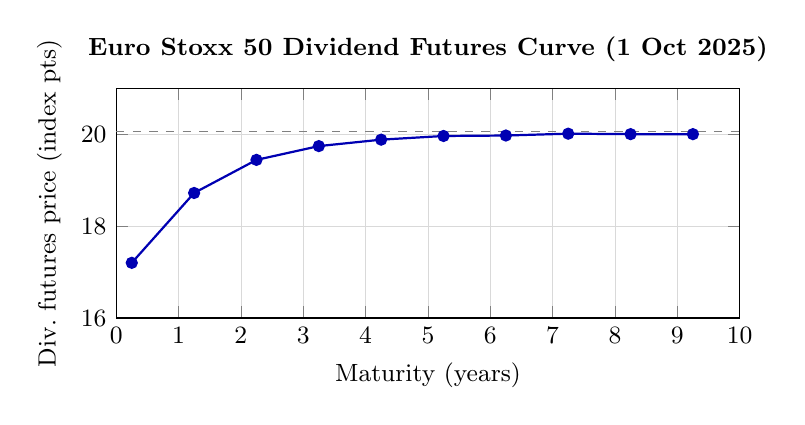
\begin{tikzpicture}
\begin{axis}[
  width=9.5cm, height=4.5cm,
  xlabel={\small Maturity (years)},
  ylabel={\small Div.\ futures price (index pts)},
  xmin=0, xmax=10, ymin=16, ymax=21,
  grid=both, grid style={line width=0.2pt, draw=gray!30},
  xtick={0,1,...,10},
  tick label style={font=\small},
  label style={font=\small},
  title style={font=\small\bfseries},
  title={Euro Stoxx 50 Dividend Futures Curve (1 Oct 2025)},
]
% Data from Table 1 of the assignment
\addplot[thick, color=blue!70!black, mark=*, mark size=1.8pt]
  coordinates {
    (0.25,17.20)(1.25,18.72)(2.25,19.44)(3.25,19.74)(4.25,19.88)
    (5.25,19.96)(6.25,19.97)(7.25,20.01)(8.25,20.00)(9.25,20.00)
  };
\draw[dashed, gray] (axis cs:0,20.05) -- (axis cs:10,20.05)
  node[right, font=\tiny, gray]{$C^*$};
\end{axis}
\end{tikzpicture}
\end{center}
 
\vspace{-4pt}
The curve observed on 1 October 2025 (plotted above using the data from Table~1) is
\emph{upward-sloping} and concave, converging toward a plateau near 20.
This shape is consistent with a mean-reverting dividend rate: near-term dividends are
priced below their long-run level (reflecting current macro caution), while the market
expects a gradual normalisation.
Structurally:
 
\begin{itemize}\setlength\itemsep{1pt}
  \item The \textbf{short end} reflects current, observable payout intentions and
    near-term corporate guidance; it is sensitive to earnings revisions.
  \item The \textbf{long end} reflects the market's view of the long-run sustainable
    dividend level, anchored by structural payout ratios; it is less volatile and more
    sensitive to long-term growth expectations.
  \item The \textbf{slope} carries information about the dividend risk premium and
    mean-reversion speed, in the same way that the slope of the yield curve reflects
    rate expectations and term premia.
\end{itemize}
 
Dividend futures are therefore the primary tool for \emph{reading and trading} this
term structure, complementing the information embedded in standard equity index options
and enriching the set of instruments available for constructing and hedging
dividend-sensitive payoffs.

\newpage

\section*{Part 2 --- Model-Free Pricing}

\subsection*{Question 1}

We aim to show that, for any strike $k$:
\begin{equation*}
\mathcal{D}_t(T) = S_t - k\,B_t(T) - C_t(T,k) + P_t(T,k)
\end{equation*}
where $\mathcal{D}_t(T)$ denotes the time-$t$ market value of dividends paid by the index over $[t, T]$.

Starting from the algebraic identity at maturity $S_T - k = (S_T - k)^+ - (k - S_T)^+$, we discount by $e^{-r(T-t)}$ and take the risk-neutral expectation $\mathbb{E}^{\mathbb{Q}}_{t}[\,\cdot\,]$. By definition of European option prices, this gives:
\begin{equation}
\mathbb{E}^{\mathbb{Q}}_{t}\!\left[e^{-r(T-t)}S_T\right] - k\,B_t(T) = C_t(T,k) - P_t(T,k) \label{eq:Q1-parity}
\end{equation}

Here $\mathcal{D}_t(T)$ is the present value of the dividends paid over $[t,T]$ (a discounted sum of cash flows in the discrete case), so that the spot price net of these dividends equals the discounted expected terminal price:
\[
\mathcal{D}_t(T) = \mathbb{E}^{\mathbb{Q}}_{t}\!\left[\sum_{n=1}^{N} {1}_{\{t < \tau_n \leq T\}} e^{-r(\tau_n - t)} d_n\right] \hspace{0.8cm} \text{(in the discrete case)}
\]
\begin{equation}
S_t - \mathcal{D}_t(T) = \mathbb{E}^{\mathbb{Q}}_{t}\!\left[e^{-r(T-t)}S_T\right] \label{eq:Q1-forward}
\end{equation}

Substituting \eqref{eq:Q1-forward} into \eqref{eq:Q1-parity} and rearranging isolates $\mathcal{D}_t(T)$:
\begin{equation*}
\boxed{\,\mathcal{D}_t(T) = S_t - k\,B_t(T) - C_t(T,k) + P_t(T,k)\,} \qquad \forall k. \qquad \square
\end{equation*}

\subsection*{Question 2}

We now show that $\mathcal{D}_t(T)$ indeed corresponds to the expected discounted dividends:
\begin{equation*}
\mathcal{D}_t(T) = \mathbb{E}^{\mathbb{Q}}_{t}\!\left[\int_{t}^{T} e^{-r(s-t)}\,dD_s\right]
\end{equation*}

Under $\mathbb{Q}$, the discounted gain process $M_t = e^{-rt}S_t + \int_{0}^{t} e^{-rs}\,dD_s$ must be a martingale. Applying $\mathbb{E}^{\mathbb{Q}}_{t}[M_T] = M_t$ yields:
\begin{equation*}
\mathbb{E}^{\mathbb{Q}}_{t}\!\left[e^{-rT}S_T + \int_{0}^{T} e^{-rs}\,dD_s\right] = e^{-rt}S_t + \int_{0}^{t} e^{-rs}\,dD_s
\end{equation*}

Splitting the integral as $\int_{0}^{T} = \int_{0}^{t} + \int_{t}^{T}$, the $\mathcal{F}_t$-measurable part $\int_{0}^{t}$ cancels out on both sides:
\begin{equation*}
\mathbb{E}^{\mathbb{Q}}_{t}\!\left[e^{-rT}S_T\right] + \mathbb{E}^{\mathbb{Q}}_{t}\!\left[\int_{t}^{T} e^{-rs}\,dD_s\right] = e^{-rt}S_t
\end{equation*}

Multiplying by $e^{rt}$ and rearranging gives:
\begin{equation*}
\mathbb{E}^{\mathbb{Q}}_{t}\!\left[\int_{t}^{T} e^{-r(s-t)}\,dD_s\right] = S_t - \mathbb{E}^{\mathbb{Q}}_{t}\!\left[e^{-r(T-t)}S_T\right]
\end{equation*}

By equation \eqref{eq:Q1-forward} from Question 1, the right-hand side is exactly $\mathcal{D}_t(T)$. Thus:
\begin{equation*}
\boxed{\,\mathcal{D}_t(T) = \mathbb{E}^{\mathbb{Q}}_{t}\!\left[\int_{t}^{T} e^{-r(s-t)}\,dD_s\right]\,} \qquad \square
\end{equation*}

This confirms the model-free equivalence between the operational definition (via market prices of a single put-call pair) and the theoretical expectation of dividends over $[t,T]$.

\subsection*{Question 3}

We need to construct a portfolio at time $t$ whose value at time $T_0$ is exactly $\mathcal{D}_{T_0}(T_1)$.

From Question 1, evaluated at time $T_0$ with maturity $T_1$ and an arbitrary strike $k_1$:
\begin{equation}
\mathcal{D}_{T_0}(T_1) = S_{T_0} - k_1\,B_{T_0}(T_1) - C_{T_0}(T_1,k_1) + P_{T_0}(T_1,k_1) \label{eq:Q3-target}
\end{equation}

The terms $-k_1\,B_{T_0}(T_1) - C_{T_0}(T_1,k_1) + P_{T_0}(T_1,k_1)$ can be straightforwardly obtained by holding the corresponding assets from time $t$:
\begin{itemize}
    \item \textbf{Short} $k_1$ units of the zero-coupon bond maturing at $T_1$.
    \item \textbf{Short} 1 call option maturing at $T_1$ with strike $k_1$.
    \item \textbf{Buy} 1 put option maturing at $T_1$ with strike $k_1$.
\end{itemize}

The remaining term is the spot price $S_{T_0}$. We cannot simply buy 1 unit of the index at time $t$, because holding the physical index would accumulate unwanted cash dividends between $t$ and $T_0$. Instead, we synthesize $S_{T_0}$ using options maturing at $T_0$. By put-call parity at $T_0$ with another arbitrary strike $k_0$:
\begin{equation*}
S_{T_0} - k_0 = C_{T_0}(T_0,k_0) - P_{T_0}(T_0,k_0) \implies S_{T_0} = C_{T_0}(T_0,k_0) - P_{T_0}(T_0,k_0) + k_0
\end{equation*}

Since $k_0$ is a guaranteed cash amount at $T_0$, it is equivalent to holding $k_0$ units of a zero-coupon bond $B(T_0)$. We thus add to our portfolio:
\begin{itemize}
    \item \textbf{Buy} 1 call option maturing at $T_0$ with strike $k_0$.
    \item \textbf{Short} 1 put option maturing at $T_0$ with strike $k_0$.
    \item \textbf{Buy} $k_0$ units of the zero-coupon bond maturing at $T_0$.
\end{itemize}

\textbf{Conclusion:} The final replicating portfolio constructed at time $t$, for any arbitrary strikes $k_0, k_1$, consists of:
\begin{table}[h]
\centering
\begin{tabular}{ll}
\textbf{Quantity} & \textbf{Asset} \\
\hline
$+1$ & Call $(T_0, k_0)$ \\
$-1$ & Put $(T_0, k_0)$ \\
$+k_0$ & Zero-coupon Bond $B(T_0)$ \\
$-1$ & Call $(T_1, k_1)$ \\
$+1$ & Put $(T_1, k_1)$ \\
$-k_1$ & Zero-coupon Bond $B(T_1)$ \\
\hline
\end{tabular}
\end{table}

At $T_0$, the $T_0$-maturity assets sum to $S_{T_0}$, and the $T_1$-maturity assets provide the remaining terms, yielding exactly $\mathcal{D}_{T_0}(T_1)$.

\subsection*{Question 4}

We aim to evaluate $\mathcal{D}^*_{T_0}(T_1) := \mathbb{E}^\mathbb{Q}_{T_0}\left[ \int_{T_0}^{T_1} dD_s \right] = \mathbb{E}^\mathbb{Q}_{T_0}\left[ D_{T_1} - D_{T_0} \right]$ and price the dividend future via a replicating portfolio $X_s$.

We rewrite the dividend integral by introducing a discount factor:
\begin{equation*}
\int_{T_0}^{T_1} dD_s = \int_{T_0}^{T_1} e^{r(s-T_0)} \left(e^{-r(s-T_0)} \,dD_s\right)
\end{equation*}
\paragraph{Discrete-to-continuous derivation of integration by parts.}
On a partition $T_0 = t_0 < \cdots < t_n = T_1$, set $\Delta V_i := V_{t_{i+1}} - V_{t_i}$ and $\Delta u_i := u_{t_{i+1}} - u_{t_i}$. Adding and subtracting $u_{t_i}V_{t_{i+1}}$ in $\Delta(uV)_i$ gives $u_{t_i}\Delta V_i = \Delta(uV)_i - V_{t_{i+1}}\Delta u_i$; summing over $i$ telescopes the product term:
\[
\sum_{i=0}^{n-1} u_{t_i}\Delta V_i = u_{t_n}V_{t_n} - u_{t_0}V_{t_0} - \sum_{i=0}^{n-1} V_{t_{i+1}}\Delta u_i .
\]
Letting the mesh $\to 0$ yields the integration-by-parts formula
\[
\int_{T_0}^{T_1} u(s)\, dV(s) = u(T_1)V(T_1) - u(T_0)V(T_0) - \int_{T_0}^{T_1} V(s)\, du(s).
\]

\paragraph{Back to our case.}
Applying integration by parts to $u(s) = e^{r(s-T_0)}$ and $V(s) = \int_{T_0}^s e^{-r(u-T_0)}dD_u$ (with therefore $V(T_0) = 0$), taking $\mathbb{E}^\mathbb{Q}_{T_0}[\,\cdot\,]$, and using Fubini's theorem:
\begin{equation}
\mathcal{D}^*_{T_0}(T_1) = e^{r(T_1-T_0)} \mathcal{D}_{T_0}(T_1) - \int_{T_0}^{T_1} r e^{r(s-T_0)} \mathcal{D}_{T_0}(s) \,ds \label{eq:Q4-payoff}
\end{equation}
where we substituted $\mathcal{D}_{T_0}(s) = \mathbb{E}^\mathbb{Q}_{T_0}\left[ \int_{T_0}^{s} e^{-r(u-T_0)} \,dD_u \right]$ from Question 2.

Equation \eqref{eq:Q4-payoff} expresses $\mathcal{D}^*_{T_0}(T_1)$ as a linear combination of $\{\mathcal{D}_{T_0}(s)\}_{s \in [T_0, T_1]}$. Let $\Pi_t(s)$ be the portfolio from Question 3 yielding $\mathcal{D}_{T_0}(s)$ at $T_0$. We synthesize $\mathcal{D}^*_{T_0}(T_1)$ at time $T_0$ by constructing at time $t$:
\begin{itemize}
    \item $+ e^{r(T_1-T_0)}$ units of $\Pi_t(T_1)$,
    \item a continuous family of short positions: $- r e^{r(s-T_0)} \,ds$ units of $\Pi_t(s)$ for all $s \in [T_0, T_1]$.
\end{itemize}
By construction, $X_{T_0} = \mathcal{D}^*_{T_0}(T_1)$.

For $s \leq T_0$, the portfolio holds only European options and zero-coupon bonds, which generate no cash flows before $T_0$; their discounted prices are $\mathbb{Q}$-martingales, so the discounted portfolio value satisfies $e^{-rs}X_s = \mathbb{E}^\mathbb{Q}_s[e^{-rT_0}X_{T_0}]$. Combined with $F_s = \mathbb{E}^\mathbb{Q}_s[X_{T_0}]$:
\begin{equation*}
X_s = e^{-r(T_0-s)} F_s \qquad \Longleftrightarrow \qquad \boxed{\,F_s = e^{r(T_0-s)} X_s\,} \qquad \square
\end{equation*}

\subsection*{Question 5}

For $s \in (T_0, T_1]$, the dividends paid over $[T_0, s]$ are already realized and $\mathcal{F}_s$-measurable. Hence the $[T_0, T_1]$-dividend futures price splits into a known part and an expectation of the remaining dividends:
\begin{equation*}
F_s = \mathbb{E}^\mathbb{Q}_s\!\left[ \int_{T_0}^{T_1} dD_u \right] = (D_s - D_{T_0}) + \mathbb{E}^\mathbb{Q}_s\!\left[ D_{T_1} - D_s \right],
\end{equation*}
that is,
\begin{equation*}
\boxed{\,F_s = (D_s - D_{T_0}) + \mathbb{E}^\mathbb{Q}_s\!\left[\int_s^{T_1} dD_u\right].\,} \qquad \square
\end{equation*}
The remaining expectation prices the not-yet-realized dividends over $[s, T_1]$, exactly as in Question 4 applied to that interval. At $s = T_1$ it vanishes, giving $F_{T_1} = D_{T_1} - D_{T_0}$; at $s = T_0$ it equals $\mathcal{D}^*_{T_0}(T_1)$, recovering Question 4.

\subsection*{Question 6}

While the model-free approach is mathematically elegant because it relies purely on no-arbitrage arguments, it faces several severe practical limitations:

\begin{itemize}
    \item \textbf{Discrete option maturities:} Question 4 requires holding a continuous spectrum of options expiring at every $s \in [T_0, T_1]$ to compute the integral. In reality, exchange-traded options exist only for discrete, standardized maturities.
    \item \textbf{Liquidity and transaction costs:} Synthesizing the index price and dividend streams requires a massive portfolio of calls/puts. Bid-ask spreads, brokerage fees, and the illiquidity of far OTM options make this replication prohibitively expensive.
    \item \textbf{Interest rate assumptions:} The derivation relies on a continuum of zero-coupon bonds with constant $r$. Real interest rates are stochastic and the curve is not flat.
    \item \textbf{European vs. American options:} Put-call parity (Question 1) requires European options. Many equity options are American, where early exercise breaks the algebraic identity.
    \item \textbf{Dividend timing risk:} Real dividends are discrete jumps (not continuous flows). Corporate decisions can shift declaration or ex-dates, creating jump risks a static portfolio cannot easily absorb.
\end{itemize}

\section*{Part 3 --- Model-Based Pricing}

\subsection*{Question 1}

Using a joint model is essential to ensure \textbf{internal consistency and prevent arbitrage}. Because the index and its dividends are structurally linked (as shown by $S_t - \mathcal{D}_t(T) = \mathbb{E}^{\mathbb{Q}}_t[e^{-r(T-t)}S_T]$), pricing them with separate models would yield inconsistent forward prices. Furthermore, a unified framework is strictly required for \textbf{coherent market calibration} and to accurately compute \textbf{cross-Greeks} when hedging dividend risks using standard index options.

\vspace{0.3cm}
\noindent \textbf{Model Setup.} The index price $S_t$, dividend rate $C_t$, and cumulative dividend $D_t$ jointly evolve under $\mathbb{Q}$ according to:
\begin{equation} \label{eq:model}
\begin{aligned}
    dS_t &= (rS_t - C_t)\,dt + \sigma \sqrt{C_t}\,dB^\mathbb{Q}_t \\
    dC_t &= \lambda(C^* - C_t)\,dt + \phi \sqrt{C_t}\,dB^\mathbb{Q}_t \\
    dD_t &= C_t\,dt
\end{aligned}
\end{equation}
where $B^\mathbb{Q}_t$ is a standard Brownian motion under $\mathbb{Q}$, and $r, \lambda, C^* > 0$ with $\phi^2 < 2\lambda C^*$ (Feller condition, ensuring $C_t > 0$). $C_t$ follows a Cox–Ingersoll–Ross (CIR) process~\cite{cir}.

\subsection*{Question 2}

\paragraph{Part 1: Expectation of $C_s$.}
We apply Itô's lemma to $f(t, C_t) = e^{\lambda t} C_t$:
\begin{align*}
    d(e^{\lambda t} C_t) &= \lambda e^{\lambda t} C_t\,dt + e^{\lambda t}\,dC_t \\
    &= \lambda e^{\lambda t} C_t\,dt + e^{\lambda t} \big(\lambda(C^* - C_t)\,dt + \phi \sqrt{C_t}\,dB^\mathbb{Q}_t\big) \\
    &= \lambda C^* e^{\lambda t}\,dt + \phi e^{\lambda t} \sqrt{C_t}\,dB^\mathbb{Q}_t
\end{align*}

Integrating from $t$ to $s$ and taking $\mathbb{E}_t^\mathbb{Q}[\cdot]$ (the Itô integral $\int_t^s \phi e^{\lambda u}\sqrt{C_u}\,dB_u^\mathbb{Q}$ is a true martingale, hence vanishes):
\begin{equation*}
    e^{\lambda s}\,\mathbb{E}_t^\mathbb{Q}[C_s] = e^{\lambda t} C_t + \lambda C^* \int_t^s e^{\lambda u}\,du = e^{\lambda t} C_t + C^*\big(e^{\lambda s} - e^{\lambda t}\big).
\end{equation*}
Dividing by $e^{\lambda s}$:
\begin{equation}
    \boxed{\,\mathbb{E}_t^\mathbb{Q}[C_s] = C^* + e^{-\lambda(s-t)}(C_t - C^*)\,} \label{eq:expected_C}
\end{equation}

\paragraph{Part 2: First martingale $\int_0^t e^{-rs}\sqrt{C_s}\,dB^{\mathbb{Q}}_s$.}
Any Itô integral $\int_0^t H_s\,dB^{\mathbb{Q}}_s$ is a true martingale under $\mathbb{Q}$ provided the $L^2$ integrability condition $\mathbb{E}^{\mathbb{Q}}\left[\int_0^t H_s^2\,ds\right] < \infty$ holds. Here, $H_s = e^{-rs}\sqrt{C_s}$, so:
\begin{equation*}
    \mathbb{E}^{\mathbb{Q}}\!\left[\int_0^t e^{-2rs} C_s\,ds\right] = \int_0^t e^{-2rs} \mathbb{E}^{\mathbb{Q}}[C_s]\,ds = \int_0^t e^{-2rs}\big[C^* + e^{-\lambda s}(C_0 - C^*)\big]\,ds
\end{equation*}
Both terms are bounded since $e^{-2rs}$ decays exponentially. Hence $\int_0^t e^{-2rs}C_s\,ds < \infty$ a.s. and in expectation, so $\int_0^t e^{-rs}\sqrt{C_s}\,dB^{\mathbb{Q}}_s$ is a true $\mathbb{Q}$-martingale. $\square$

\paragraph{Part 3: Second martingale  discounted gain process $N_t = e^{-rt}S_t + \int_0^t e^{-rs}C_s\,ds$.}
Applying Itô's lemma to $e^{-rt} S_t$:
\begin{align*}
    d(e^{-rt} S_t) &= -r e^{-rt} S_t\,dt + e^{-rt}\,dS_t \\
    &= -r e^{-rt} S_t\,dt + e^{-rt} \big((rS_t - C_t)\,dt + \sigma \sqrt{C_t}\,dB^{\mathbb{Q}}_t\big) \\
    &= -e^{-rt} C_t\,dt + \sigma e^{-rt} \sqrt{C_t}\,dB^{\mathbb{Q}}_t
\end{align*}

Therefore:
\begin{equation*}
    dN_t = d(e^{-rt} S_t) + e^{-rt} C_t\,dt = \sigma e^{-rt} \sqrt{C_t}\,dB^{\mathbb{Q}}_t
\end{equation*}
\begin{equation*}
    N_t = N_0 + \sigma \int_0^t e^{-rs}\sqrt{C_s}\,dB^{\mathbb{Q}}_s
\end{equation*}

Since $\int_0^t e^{-rs}\sqrt{C_s}\,dB^{\mathbb{Q}}_s$ is a true martingale (Part 2), so is $N_t$. $\square$

\subsection*{Question 3}

We evaluate $F_t := \mathbb{E}^{\mathbb{Q}}_t \left[ \int_t^\infty e^{-r(s-t)} C_s \,ds \right]$. By Fubini and \eqref{eq:expected_C}:
\begin{align*}
    F_t &= \int_t^\infty e^{-r(s-t)} \mathbb{E}^{\mathbb{Q}}_t[C_s] \,ds = C^* \int_t^\infty e^{-r(s-t)}\,ds + (C_t - C^*) \int_t^\infty e^{-(r+\lambda)(s-t)}\,ds \\
    &= \frac{C^*}{r} + \frac{C_t - C^*}{r+\lambda}
\end{align*}

This matches the form $F_t = a + b(C_t - C^*)$ with:
\begin{equation*}
    \boxed{\,a = \frac{C^*}{r}, \qquad b = \frac{1}{r+\lambda}\,}
\end{equation*}

\paragraph{Interpretation.} The dividend rate $C_t$ represents a continuous flow of dividends per unit of time. The price $F_t$ is therefore the present value of an infinite stream of infinitesimal dividend payments $C_s ds$, each discounted at rate $r$.

Equivalently, $F_t$ can be interpreted as the fundamental value of the index, i.e. the discounted expected value of all future dividend flows.

If the price is fully determined by fundamentals, meaning that no additional non-fundamental component enters the valuation, then the index price satisfies
\[
S_t = F_t,
\]
as established in Question 4.

\subsection*{Question 4}

\paragraph{Part 1: The pricing identity.}
From Question 2, $N_t$ is a true $\mathbb{Q}$-martingale, so $\mathbb{E}^{\mathbb{Q}}_t[N_T] = N_t$:
\begin{equation*}
    e^{-rt}S_t + \int_0^t e^{-rs}C_s\,ds = \mathbb{E}^{\mathbb{Q}}_t\left[e^{-rT}S_T + \int_0^T e^{-rs}C_s\,ds\right]
\end{equation*}
Cancelling the $\mathcal{F}_t$-measurable $\int_0^t$ term and multiplying by $e^{rt}$:
\begin{equation}
    \boxed{\,S_t = \mathbb{E}^{\mathbb{Q}}_t\!\left[ e^{-r(T-t)} S_T \right] + \mathbb{E}^{\mathbb{Q}}_t\!\left[ \int_t^T e^{-r(s-t)} C_s \,ds \right]\,} \label{eq:Q4-spot}
\end{equation}

\paragraph{Part 2: Equivalence of (a), (b), (c).}
The three properties to be shown equivalent are: \textbf{(a)} $\sigma = \frac{\phi}{r+\lambda}$ \emph{and} $S_0 = F_0$;\quad \textbf{(b)} $S_t = F_t$ for all $t \geq 0$;\quad \textbf{(c)} $\lim_{T\to\infty}\mathbb{E}^{\mathbb{Q}}_t[e^{-r(T-t)}S_T] = 0$ for all $t \geq 0$.

Taking $T \to \infty$ in \eqref{eq:Q4-spot}, the dividend integral converges to $F_t$:
\begin{equation}
    S_t = \lim_{T \to \infty} \mathbb{E}^{\mathbb{Q}}_t\!\left[ e^{-r(T-t)} S_T \right] + F_t \label{eq:Q4-limit}
\end{equation}

\noindent\textbf{(b) $\Leftrightarrow$ (c).} If $S_t = F_t$ (b), then the limit in \eqref{eq:Q4-limit} is zero (c). Conversely, if (c), then $S_t = F_t$ (b).

\noindent\textbf{(a) $\Rightarrow$ (b)+(c).} Assume $\sigma = \phi/(r+\lambda)$ \emph{and} $S_0 = F_0$. Define $\Delta_t := S_t - F_t$, so that $\Delta_0 = S_0 - F_0 = 0$. By Itô on $F_t = \frac{C^*}{r} + \frac{C_t - C^*}{r+\lambda}$:
\begin{equation*}
    dF_t = \frac{1}{r+\lambda}dC_t = \frac{\lambda}{r+\lambda}(C^* - C_t)\,dt + \frac{\phi}{r+\lambda}\sqrt{C_t}\,dB^{\mathbb{Q}}_t
\end{equation*}
Subtracting from $dS_t$:
\begin{equation*}
    d\Delta_t = \left(rS_t - C_t - \frac{\lambda}{r+\lambda}(C^* - C_t)\right)dt + \underbrace{\left(\sigma - \frac{\phi}{r+\lambda}\right)}_{=0}\sqrt{C_t}\,dB^{\mathbb{Q}}_t
\end{equation*}
The diffusion term vanishes by the first part of (a). The drift simplifies to $rS_t - C_t - \frac{\lambda(C^*-C_t)}{r+\lambda} = r\big[S_t - F_t\big] = r\Delta_t$, so $d\Delta_t = r\Delta_t\,dt$, giving $\Delta_t = \Delta_0 e^{rt}$. By the second part of (a), $\Delta_0 = 0$, hence $\Delta_t \equiv 0$, i.e. $S_t = F_t$ (b). Substituting into \eqref{eq:Q4-limit} then gives $\lim_{T\to\infty}\mathbb{E}^{\mathbb{Q}}_t[e^{-r(T-t)}S_T] = S_t - F_t = 0$ (c).

\noindent\textbf{(b) $\Rightarrow$ (a).} If $S_t = F_t$ for all $t$, matching diffusion terms of $dS_t$ and $dF_t$ gives $\sigma\sqrt{C_t} = \frac{\phi}{r+\lambda}\sqrt{C_t}$, i.e. $\sigma = \phi/(r+\lambda)$; and $S_0 = F_0$ holds as the $t=0$ instance of (b). Both parts of (a) hold.

All three properties are therefore equivalent. $\square$

\subsection*{Question 5}

\paragraph{Boundedness of $\delta_t$.}
From (b), $S_t = \alpha + \beta C_t$ where $\alpha = \frac{\lambda C^*}{r(r+\lambda)} > 0$ and $\beta = \frac{1}{r+\lambda} > 0$. The dividend yield is:
\begin{equation*}
    \delta_t = \frac{C_t}{S_t} = \frac{C_t}{\alpha + \beta C_t}
\end{equation*}
$\delta_t$ is monotonically increasing in $C_t$, with $\delta_t \to 0$ as $C_t \to 0^+$ and $\delta_t \to 1/\beta = r+\lambda$ as $C_t \to \infty$. Hence $\delta_t \in (0, r+\lambda)$ is bounded.

\paragraph{Autonomous SDE for $\delta_t$.}
Inverting: $C_t = \alpha\delta_t/(1 - \beta\delta_t)$. Apply Itô to $\delta_t = f(C_t)$ with $f(c) = c/(\alpha + \beta c)$:
\begin{equation*}
    f'(c) = \frac{\alpha}{(\alpha + \beta c)^2}, \qquad f''(c) = -\frac{2\alpha\beta}{(\alpha + \beta c)^3}
\end{equation*}

Using the identity $(\alpha + \beta C_t)^{-1} = (1 - \beta\delta_t)/\alpha$, we obtain:
\begin{equation*}
    f'(C_t) = \frac{(1-\beta\delta_t)^2}{\alpha}, \qquad C_t f'(C_t) = \delta_t(1-\beta\delta_t), \qquad C_t f''(C_t) = -\frac{2\beta\delta_t(1-\beta\delta_t)^2}{\alpha}
\end{equation*}

Substituting into Itô's formula (with $dC_t = \lambda(C^* - C_t)dt + \phi\sqrt{C_t}dB^{\mathbb{Q}}_t$ and $d\langle C\rangle_t = \phi^2 C_t\,dt$):
\begin{align*}
    d\delta_t &= \big[\lambda(C^* - C_t)f'(C_t) + \tfrac{1}{2}\phi^2 C_t f''(C_t)\big]dt + \phi\sqrt{C_t}\,f'(C_t)\,dB^{\mathbb{Q}}_t \\
    &= \frac{(1-\beta\delta_t)^2}{\alpha}\!\left[\lambda(C^* - C_t) - \phi^2 \beta \delta_t\right]\!dt + \phi\sqrt{C_t}\,\frac{(1-\beta\delta_t)^2}{\alpha}\,dB^{\mathbb{Q}}_t
\end{align*}
where we used $f'(C_t)=\frac{(1-\beta\delta_t)^2}{\alpha}$ together with $\tfrac{1}{2}\phi^2 C_t f''(C_t) = -\frac{\phi^2\beta\delta_t(1-\beta\delta_t)^2}{\alpha} = -\phi^2\beta\delta_t\,f'(C_t)$ (sharing the same factor $f'(C_t)$). Substituting $C_t = \alpha\delta_t/(1-\beta\delta_t)$ in both terms:
\begin{equation*}
    \boxed{\,d\delta_t = (1-\beta\delta_t)^2\!\left[\frac{\lambda C^*}{\alpha} - \frac{\lambda \delta_t}{1-\beta\delta_t} - \frac{\phi^2 \beta \delta_t}{\alpha}\right]\!dt + \frac{\phi\,(1-\beta\delta_t)^{3/2}\sqrt{\delta_t}}{\sqrt{\alpha}}\,dB^{\mathbb{Q}}_t\,}
\end{equation*}
with $\alpha=\frac{\lambda C^*}{r(r+\lambda)}$ and $\beta=\frac{1}{r+\lambda}$. Every coefficient depends only on $\delta_t$ and the constants $(r,\lambda,\phi,C^*)$, confirming that $\delta_t$ is an autonomous Markov diffusion.
\subsection*{Question 6}

Since $r$ is constant, $F(t,T) = \mathbb{E}^{\mathbb{Q}}_t[S_T]$. Using $S_T = F_T = \frac{C^*}{r} + \frac{C_T - C^*}{r+\lambda}$ and \eqref{eq:expected_C}:
\begin{align*}
    F(t,T) &= \frac{C^*}{r} + \frac{\mathbb{E}^{\mathbb{Q}}_t[C_T] - C^*}{r+\lambda} = \frac{C^*}{r} + e^{-\lambda(T-t)}\frac{C_t - C^*}{r+\lambda}
\end{align*}

Recognizing $S_t = \frac{C^*}{r} + \frac{C_t - C^*}{r+\lambda}$:
\begin{equation*}
    \boxed{\,F(t,T) = \frac{C^*}{r}\big(1 - e^{-\lambda(T-t)}\big) + S_t\,e^{-\lambda(T-t)}\,} \qquad \square
\end{equation*}
\textit{The futures price is a weighted average between the long-term fundamental value $C^*/r$ and the current spot $S_t$.}

\subsection*{Question 7}

Let $\tau = t \vee T_0 = \max\{t, T_0\}$. The dividend futures price is:
\begin{equation*}
    F_t^{div} = \mathbb{E}^{\mathbb{Q}}_t\!\left[\int_{T_0}^{T_1} C_s\,ds\right] = (D_\tau - D_{T_0}) + \int_\tau^{T_1} \mathbb{E}^{\mathbb{Q}}_t[C_s]\,ds
\end{equation*}

The first term is the realized cumulative dividend, $\mathcal{F}_t$-measurable. For the second, using \eqref{eq:expected_C}:
\begin{equation*}
    \int_\tau^{T_1} \big(C^* + e^{-\lambda(s-t)}(C_t - C^*)\big)ds = C^*(T_1 - \tau) + \frac{C_t - C^*}{\lambda}\big(e^{-\lambda(\tau-t)} - e^{-\lambda(T_1-t)}\big)
\end{equation*}

Combining:
\begin{equation*}
    \boxed{\,F_t^{div} = (D_\tau - D_{T_0}) + C^*(T_1 - \tau) + \frac{C_t - C^*}{\lambda}\!\left(e^{-\lambda(\tau-t)} - e^{-\lambda(T_1-t)}\right)\,} \qquad \square
\end{equation*}

\subsection*{Question 8}

\paragraph{Part 1: Expectation of $e^{-w C_{T_1}}$.}
Let
\[
V(t, C) = \mathbb{E}^{\mathbb{Q}}_t \left[e^{-w C_{T_1}}\right].
\]
By Feynman-Kac, $V$ satisfies:
\begin{equation*}
    \frac{\partial V}{\partial t}
    + \lambda(C^* - C)\frac{\partial V}{\partial C}
    + \tfrac{1}{2}\phi^2 C\,\frac{\partial^2 V}{\partial C^2}
    = 0,
    \qquad
    V(T_1, C) = e^{-wC}.
\end{equation*}
Hence the PDE becomes:
\[
\frac{\partial V}{\partial t}
+ \lambda C^*\frac{\partial V}{\partial C}
+ \left(
-\lambda \frac{\partial V}{\partial C}
+ \tfrac{1}{2}\phi^2 \frac{\partial^2 V}{\partial C^2}
\right) C
= 0.
\]
Guessing the affine form $V(t,C) = e^{-a_0(T_1-t) - b_0(T_1-t)C}$ with $\theta = T_1 - t$, we have
\begin{align*}
\frac{\partial V}{\partial C}
&= -b_0(\theta)\,V(t,C), \\
\frac{\partial^2 V}{\partial C^2}
&= b_0(\theta)^2\,V(t,C), \\
\frac{\partial V}{\partial t}
&= \left(a_0'(\theta) + b_0'(\theta)C\right)V(t,C).
\end{align*}
Substituting into the PDE and dividing by $V(t,C)$ (which is always non-zero), we obtain:
\[
a_0'(\theta) + b_0'(\theta)C
+ \lambda C^*(-b_0(\theta))
+ \left(
-\lambda(-b_0(\theta))
+ \tfrac{1}{2}\phi^2 b_0(\theta)^2
\right) C
= 0.
\]
We now separate constant and $C$ terms.
\paragraph{Constant term:}
\[
a_0'(\theta) - \lambda C^* b_0(\theta) = 0.
\]
\paragraph{$C$-term:}
\[
b_0'(\theta) + \lambda b_0(\theta) + \tfrac{1}{2}\phi^2 b_0(\theta)^2 = 0.
\]
Thus we obtain the ODE system:
\begin{equation*}
    \boxed{
    \begin{cases}
        b_0'(\theta) = -\lambda b_0(\theta) - \tfrac{1}{2}\phi^2 b_0(\theta)^2 \\
        a_0'(\theta) = \lambda C^* b_0(\theta)
    \end{cases}
    }
\end{equation*}
with boundary conditions:
\[
b_0(0) = w, \qquad a_0(0) = 0.
\]
The functions $a_0$ and $b_0$ depend on $w$ through the initial condition $b_0(0) = w$; they are \emph{determined} as the unique solutions of this Riccati system (the homogeneous $b_0$-equation is a Bernoulli ODE, solvable in closed form).

\paragraph{Part 2: Expectation of $e^{-w(D_{T_1} - D_{T_0})}$.}
Let $\tau = t \vee T_0 = \max\{t,T_0\}$. We decompose the increment:
\[
D_{T_1} - D_{T_0}
=
(D_\tau - D_{T_0}) + \int_\tau^{T_1} C_s\,ds.
\]
The first term equals $D_t - D_{T_0}$ if $t \ge T_0$ and $0$ if $t < T_0$; in both cases it is $\mathcal{F}_t$-measurable and equal to $D_{t\vee T_0} - D_{T_0}$, so:
\begin{equation}
\mathbb{E}^{\mathbb{Q}}_t\!\left[e^{-w(D_{T_1} - D_{T_0})}\right]
=
e^{-w(D_{t\vee T_0} - D_{T_0})}
\,
\mathbb{E}^{\mathbb{Q}}_t\!\left[e^{-w\int_\tau^{T_1} C_s\,ds}\right]. \label{eq:Q8-factor}
\end{equation}
We first solve the running-cost (source) problem. Define
\[
U(\tau, C)
=
\mathbb{E}^{\mathbb{Q}}_\tau\!\left[e^{-w\int_\tau^{T_1} C_s\,ds}\right].
\]
By Feynman-Kac with running cost $-wC$, $U$ satisfies
\begin{equation*}
\frac{\partial U}{\partial \tau}
+ \lambda(C^* - C)\frac{\partial U}{\partial C}
+ \tfrac{1}{2}\phi^2 C \frac{\partial^2 U}{\partial C^2}
- wC\,U
= 0,
\qquad
U(T_1, C) = 1.
\end{equation*}
With the affine ansatz $U(\tau,C) = \exp(-\bar a(\eta) - \bar b(\eta)C)$, $\eta = T_1 - \tau$, we have $\partial_C U = -\bar b\,U$, $\partial_{CC} U = \bar b^2 U$ and $\partial_\tau U = (\bar a'(\eta) + \bar b'(\eta)C)U$ (the sign arising from $\eta = T_1-\tau$). Substituting and dividing by $U$:
\[
\bar a'(\eta) + \bar b'(\eta)C - \lambda C^* \bar b(\eta) + \left(\lambda \bar b(\eta) + \tfrac{1}{2}\phi^2 \bar b(\eta)^2 - w\right)C = 0.
\]
Separating the constant and $C$ terms yields the ODE system
\begin{equation*}
\boxed{
\begin{cases}
\bar b'(\eta) = -\lambda \bar b(\eta) - \tfrac{1}{2}\phi^2 \bar b(\eta)^2 + w \\
\bar a'(\eta) = \lambda C^* \bar b(\eta)
\end{cases}
}
\qquad \bar b(0)=0, \quad \bar a(0)=0.
\end{equation*}

\noindent\textbf{Case 1: $T_0 \le t \le T_1$ (so $\tau = t$).} The inner expectation in \eqref{eq:Q8-factor} is directly $U(t,C_t)$, hence
\begin{equation*}
\mathbb{E}^{\mathbb{Q}}_t\!\left[e^{-w(D_{T_1} - D_{T_0})}\right]
= e^{-\bar a(T_1-t) - \bar b(T_1-t)C_t - w(D_t - D_{T_0})}.
\end{equation*}

\noindent\textbf{Case 2: $0 \le t < T_0$ (so $\tau = T_0$).} Here $C_t$ is not the state at the start of the window $[T_0,T_1]$, so we evaluate $U$ at $T_0$ and propagate back to $t$. By the tower and Markov properties,
\begin{equation*}
\mathbb{E}^{\mathbb{Q}}_t\!\left[e^{-w\int_{T_0}^{T_1}C_s\,ds}\right]
= \mathbb{E}^{\mathbb{Q}}_t\!\left[U(T_0,C_{T_0})\right]
= e^{-\bar a(T_1-T_0)}\;\mathbb{E}^{\mathbb{Q}}_t\!\left[e^{-\bar b(T_1-T_0)\,C_{T_0}}\right].
\end{equation*}
The last factor is exactly of the Part~1 type, with exponent $\tilde{w} := \bar b(T_1-T_0) \ge 0$ and horizon $T_0$. Reusing the source-free functions $a_0,b_0$ of Part~1 (same ODEs), now with initial condition $b_0(0) = \tilde{w}$:
\begin{equation*}
\mathbb{E}^{\mathbb{Q}}_t\!\left[e^{-\tilde{w}\,C_{T_0}}\right]
= e^{-a_0(T_0-t) - b_0(T_0-t)C_t},
\qquad
\begin{cases}
b_0'(\theta) = -\lambda b_0(\theta) - \tfrac{1}{2}\phi^2 b_0(\theta)^2, & b_0(0)=\bar b(T_1-T_0),\\[2pt]
a_0'(\theta) = \lambda C^* b_0(\theta), & a_0(0)=0.
\end{cases}
\end{equation*}
Since $D_{t\vee T_0}-D_{T_0}=0$ in this regime,
\begin{equation*}
\mathbb{E}^{\mathbb{Q}}_t\!\left[e^{-w(D_{T_1} - D_{T_0})}\right]
= e^{-\left[\bar a(T_1-T_0) + a_0(T_0-t)\right] - b_0(T_0-t)C_t}.
\end{equation*}

\noindent\textbf{Unified form.} Both cases combine into
\begin{equation*}
\boxed{\;\mathbb{E}^{\mathbb{Q}}_t\!\left[e^{-w(D_{T_1} - D_{T_0})}\right]
= e^{-a(t) - b(t)C_t - w(D_{t\vee T_0} - D_{T_0})}\;}
\end{equation*}
with $a(t)\equiv a(t;w)$ and $b(t)\equiv b(t;w)$, where we now display the dependence on $w$ explicitly as a second argument (for $a_0,b_0$ it is their initial value $b_0(0)$):
\begin{equation*}
b(t;w)=\begin{cases} \bar b(T_1-t;w), & T_0\le t\le T_1,\\[2pt] b_0\big(T_0-t;\,\bar b(T_1-T_0;w)\big), & 0\le t<T_0,\end{cases}
\end{equation*}
\begin{equation*}
a(t;w)=\begin{cases} \bar a(T_1-t;w), & T_0\le t\le T_1,\\[2pt] \bar a(T_1-T_0;w)+a_0\big(T_0-t;\,\bar b(T_1-T_0;w)\big), & 0\le t<T_0,\end{cases}
\end{equation*}
where $\bar a(\cdot;w),\bar b(\cdot;w)$ solve the source-$w$ Riccati system (zero initial condition) and $a_0(\cdot;\beta),b_0(\cdot;\beta)$ the source-free system of Part~1 with initial value $b_0(0)=\beta$. The two branches match at $t=T_0$ (since $a_0(0;\cdot)=0$ and $b_0(0;\beta)=\beta$), so $a,b$ are continuous; and \emph{every} branch depends on $w$ --- directly through the source term for $t\ge T_0$, and through the initial value $\bar b(T_1-T_0;w)$ for $t<T_0$.

\subsection*{Question 9}

\paragraph{Part 1: Laplace transform via Fubini.}
Let $X = D_{T_1} - D_{T_0}$. We compute:
\begin{equation*}
    \hat{P}_t(w) = \int_0^\infty e^{-wk} P_t(k)\,dk = e^{-r(T_1-t)}\,\mathbb{E}^{\mathbb{Q}}_t\!\left[\int_0^\infty e^{-wk}(k - X)^+\,dk\right]
\end{equation*}
The inner integral evaluates to $e^{-wX}/w^2$ via the substitution $u = k - X$. Hence:
\begin{equation*}
    \hat{P}_t(w) = \frac{e^{-r(T_1-t)}}{w^2}\,\mathbb{E}^{\mathbb{Q}}_t[e^{-wX}]
\end{equation*}

Using Question~8 and absorbing the deterministic factor $e^{-r(T_1-t)}$ into the exponent:
\begin{equation*}
    \boxed{\,\hat{P}_t(w) = \frac{1}{w^2}\,e^{-\hat{a}(t) - \hat{b}(t)C_t - w(D_{t \vee T_0} - D_{T_0})}\,} \qquad \square
\end{equation*}
where $a(t),b(t)$ are the (piecewise) functions of Question~8 and
\[
\hat{b}(t) = b(t), \qquad \hat{a}(t) = a(t) + r(T_1 - t),
\]
the discount factor contributing only to the constant part $\hat{a}$ (it carries no $C_t$). In particular $\hat{a},\hat{b}$ inherit the two-regime structure of $a,b$ across $t \lessgtr T_0$.

\paragraph{Part 2: Numerical Inversion.}
Since $\hat{P}_t(w)$ is available in closed form, we recover $P_t(k)$ by inverting its Laplace transform numerically. The idea is to evaluate $\hat{P}_t(w)$ along a vertical line in the complex plane, $w = \alpha + iu$ with $\alpha > 0$, which ensures the integral is stable and well-behaved.
This leads to a one-dimensional integral over frequencies $u$:
\begin{equation*}
P_t(k)
= \frac{e^{\alpha k}}{\pi}
\int_0^\infty \mathrm{Re}\!\left(\hat{P}_t(\alpha + iu)\,e^{iuk}\right)du
\end{equation*}

In practice, this integral is not computed analytically but approximated numerically on a finite grid of $u$ values. Standard quadrature methods can be used (trapezoidal rule or Euler acceleration), and when many strikes are needed, the computation can be accelerated using a Fast Fourier Transform (FFT) approach.

\subsection*{Question 10}

\paragraph{Part 1: Moment-generating property.}
Differentiating $n$ times under the expectation:
\begin{equation*}
    \frac{d^n}{dw^n} \mathbb{E}^{\mathbb{Q}}_t[e^{-wX}] = \mathbb{E}^{\mathbb{Q}}_t[(-X)^n e^{-wX}] = (-1)^n \mathbb{E}^{\mathbb{Q}}_t[X^n e^{-wX}]
\end{equation*}
At $w = 0$:
\begin{equation*}
    \boxed{\,\mathbb{E}^{\mathbb{Q}}_t[(D_{T_1} - D_{T_0})^n] = (-1)^n \left.\frac{d^n}{dw^n}\mathbb{E}^{\mathbb{Q}}_t[e^{-w(D_{T_1} - D_{T_0})}]\right|_{w=0}\,}
\end{equation*}

\paragraph{Part 2: General expression for moments.}
Let $g(w) = -a(t) - b(t)C_t - w(D_\tau - D_{T_0})$ (with $\tau = t \vee T_0$), where $a(t),b(t)$ are the deterministic functions of (corrected) Question~8 at the valuation date $t$, regarded as functions of $w$; for $t \le T_0$ they are the two-regime composites derived there. Then $\mathbb{E}^{\mathbb{Q}}_t[e^{-wX}] = e^{g(w)}$ with $g(0) = 0$. We therefore have
\begin{equation*}
    \mathbb{E}^{\mathbb{Q}}_t[X^n] = (-1)^n B_n\!\big(g'(0), g''(0), \dots, g^{(n)}(0)\big)
\end{equation*}
where:
\begin{align*}
    g'(0) &= -\left.\tfrac{da}{dw}\right|_{w=0} - \left.\tfrac{db}{dw}\right|_{w=0}\!C_t - (D_\tau - D_{T_0}) \\
    g^{(k)}(0) &= -\left.\tfrac{d^ka}{dw^k}\right|_{w=0} - \left.\tfrac{d^kb}{dw^k}\right|_{w=0}\!C_t \quad (k \geq 2)
\end{align*}

\paragraph{Part 3: Futures on squared cumulative dividends ($n=2$).}
$\frac{d^2}{dw^2}e^{g(w)}\big|_{w=0} = g''(0) + g'(0)^2$, so:
\begin{equation*}
    \boxed{\,F_t^{(2)} = -\!\left.\tfrac{d^2a}{dw^2}\right|_{w=0} - \!\left.\tfrac{d^2b}{dw^2}\right|_{w=0}\!C_t + \!\left(\!\left.\tfrac{da}{dw}\right|_{w=0} + \!\left.\tfrac{db}{dw}\right|_{w=0}\!C_t + (D_\tau - D_{T_0})\!\right)^{\!2}\,} \qquad \square
\end{equation*}

\textit{The squared term equals $(F_t^{div})^2$ from Question 7. The remaining second-derivative terms represent the convexity adjustment (variance of cumulative dividends).}

\subsection*{Question 11}

\paragraph{Part 1: Density of $S_T$.}
From (b) of Question 4, $S_t = \alpha + \beta C_t$ with $\alpha = \frac{\lambda C^*}{r(r+\lambda)}$, $\beta = \frac{1}{r+\lambda}$, and $C_t = (S_t - \alpha)/\beta$. Since the map is affine with constant Jacobian $\beta$, the change of variables formula gives:
\begin{equation*}
    f_{S_T}(s) = \frac{1}{\beta}\,f_{C_T}\!\left(\frac{s - \alpha}{\beta}\right) = (r+\lambda)\,f_{C_T}\!\big((r+\lambda)(s - \alpha)\big)
\end{equation*}

Substituting the given CIR density (with $C_0 = (S_0 - \alpha)/\beta$):
\begin{equation*}
    \boxed{\,f_{S_T}(s) = (r+\lambda)\,a\,e^{-a\!\left[\frac{s-\alpha}{\beta} + e^{-\lambda T}\frac{S_0 - \alpha}{\beta}\right]}\!\left(e^{\lambda T}\,\frac{s-\alpha}{S_0 - \alpha}\right)^{\!q/2}\!\!I_q\!\left(2a\sqrt{e^{-\lambda T}\frac{(s-\alpha)(S_0-\alpha)}{\beta^2}}\right)\,}
\end{equation*}
Here $q = \frac{2\lambda C^*}{\phi^2}-1$ and $a = \frac{2\lambda}{\phi^2\left(1-e^{-\lambda T}\right)}$ are the constants of the given CIR density (this $a$ is the density constant from the statement, not the $a=C^*/r$ of Question~3), and $I_q$ is the modified Bessel function of the first kind. The density is supported on $s > \alpha = S_{\min}$ (since $C_T > 0$).

\paragraph{Part 2: Initial price of an index call.}
For a European index call with strike $K$ and maturity $T$:
\begin{equation*}
    \boxed{\,\mathrm{Call}(0, T, K) = e^{-rT}\!\int_{\max(K, S_{\min})}^\infty\!\!(s - K)\,f_{S_T}(s)\,ds\,} \qquad \square
\end{equation*}

\subsection*{Question 12}

\paragraph{Calibration setup.} We estimate $\Theta = (\lambda, C^*, C_0, \phi)$ by minimizing the unweighted SSE between market and model prices:
\begin{equation*}
    \min_\Theta \big(S_0^{\mathrm{mod}} - S_0^{\mathrm{mkt}}\big)^2 + \sum_{k=0}^9 \big(F^{\mathrm{mod}}_{div}(k) - F^{\mathrm{mkt}}_{div}(k)\big)^2 + \big(\mathrm{Call}^{\mathrm{mod}} - \mathrm{Call}^{\mathrm{mkt}}\big)^2
\end{equation*}
subject to $\lambda, C^*, C_0, \phi > 0$ and the Feller condition $2\lambda C^* > \phi^2$.

\paragraph{Implementation.} We use Python (\texttt{scipy.optimize.minimize} with SLSQP). $S_0^{\mathrm{mod}}$ and $F^{\mathrm{mod}}_{div}$ are computed via the closed-form formulas from Questions 6 and 7. The call price is computed via numerical integration of the payoff against the analytical CIR density (Question 11), with algebraic refactoring of the exponent to prevent \texttt{float64} overflow.

\paragraph{Results.} The optimization converges (SSE $\approx 0.36$):
\begin{equation*}
    \lambda = 0.5266, \quad C^* = 20.0474, \quad C_0 = 16.1972, \quad \phi = 4.5949
\end{equation*}

\paragraph{Discussion.} The long-term mean $C^* \approx 20.05$ matches the plateau of far-dated futures (Table 1), while $C_0 \approx 16.20$ reflects depressed short-term dividend expectations. The high volatility $\phi \approx 4.59$ is required to match the Black-Scholes implied volatility ($\sigma_{BS} = 4.635\%$), pushing the parameters close to the Feller boundary $2\lambda C^* = \phi^2$ ($2\lambda C^* \approx \phi^2 \approx 21.11$) --- the condition that guarantees strict positivity of the CIR process. As a result, the process frequently operates in a regime where $C_t$ can get arbitrarily close to zero, making the model numerically unstable (due to $\sqrt{C_t}$) and less reliable under stressed market conditions.

\subsection*{Question 13}

To replicate a 1Y ATM call ($T_1 = 1$) with a 2Y futures contract ($T_2 = 2$), we delta-hedge. Under property (b) of Question 4, $S_t = F_t$ implies that $C_t$ and $S_t$ are deterministically linked ($C_t = (S_t - \alpha)/\beta$); hence both the call and the futures depend on a \textbf{single state variable}, making the delta scalar.

The number of futures is:
\begin{equation*}
    n_F = \frac{\partial V(0, S_0)/\partial S_0}{\partial F(0, T_2)/\partial S_0}
\end{equation*}

From Question 6, $\partial F(0, T_2)/\partial S_0 = e^{-\lambda T_2}$. The call delta $\Delta_{\mathrm{call}}^{1Y} = \partial V(0, S_0)/\partial S_0$ is computed via central finite differences on the calibrated integral pricer (shifting $C_0$ consistently with $S_0$). Therefore:
\begin{equation*}
    \boxed{\,n_F = \Delta_{\mathrm{call}}^{1Y}\,e^{\lambda T_2}\,} \qquad \square
\end{equation*}

Numerically:
\begin{equation*}
    n_F \approx 1.0765
\end{equation*}

\textit{Interpretation: the 2Y futures is less sensitive to an immediate spot move than the spot itself ($\partial F(0,T_2)/\partial S_0 = e^{-\lambda T_2} \approx 0.35$), so each unit of call delta must be hedged with $e^{\lambda T_2} \approx 2.87$ futures; the 1Y call delta is small enough that the resulting position is only $n_F \approx 1.08$ contracts.}

\begin{thebibliography}{9}\footnotesize
\bibitem{eurex} Eurex, \emph{EURO STOXX 50 Index Dividend Futures (FEXD): Contract Specifications}, Eurex Exchange. \url{https://www.eurex.com/ex-en/markets/did}.
\bibitem{hull} J.~C. Hull, \emph{Options, Futures, and Other Derivatives}, Pearson.
\bibitem{vbk} J.~van~Binsbergen, M.~Brandt, and R.~Koijen, ``On the Timing and Pricing of Dividends,'' \emph{American Economic Review} 102(4):1596--1618, 2012.
\bibitem{cir} J.~Cox, J.~Ingersoll, and S.~Ross, ``A Theory of the Term Structure of Interest Rates,'' \emph{Econometrica} 53(2):385--407, 1985.
\end{thebibliography}

\end{document}